\documentclass[10pt,  english, makeidx, a4paper, titlepage, oneside]{book}

% Packages
\usepackage{graphicx} % Usato per \includegraphics 
\usepackage{titlesec} % Usato per modificare/rimuovere le scritte Capitolo 1,2 ecc
\usepackage{textcomp} % Per caratteri speciali
\usepackage{listings} % Per VHDL
%\usepackage[sfdefault]{Roboto}  
%\usepackage[T1]{fontenc}

% Impostazioni pagina
\textwidth 15.5cm % larghezza del testo nella pagina
\textheight 23cm % altezza del testo nella pagina
\topmargin -2cm % spazio in più o in meno dall'alto
\oddsidemargin 0cm % si può spostare il margine dove inizia il testo nella pagina 
\titleformat{\chapter}[display]
{\normalfont\bfseries}{}{0pt}{\Huge} % Rimuove le scritte Capitolo 1,2 ecc
\newenvironment{listato}{\footnotesize}
                        {\normalsize }




% inizio del documento
\begin{document}

% pagina iniziale
\begin{titlepage}

	\centerline{
\includegraphics[width=3cm]{./img/general/polito.png}}
	\vspace{0.3cm}
	\centerline{\Large{Politecnico di Torino}}
	\vspace{0.3cm}
	\centerline{\Large{III Facoltà di Ingegneria}}
	\vspace{3cm}
	\centerline{\Huge\textbf{Sistemi elettronici a basso consumo}}
	\vspace{1cm}
	\centerline{\LARGE\textbf{Relazioni di laboratorio}}
	\vspace{3cm}
	\centerline{\LARGE{Laurea Magistrale in Ingegneria Elettronica}}
	\vspace{0.3cm}
	\centerline{\LARGE{Orientamento: Sistemi Elettronici}}
	\vspace{3cm}
	\centerline{\Large{Gruppo n. 9}}
	\vspace{2cm}
	\centerline{\Large{Autori:}}
	\vspace{0.3cm}
	\centerline{\Large{Favero Simone, Micelli Federico, Spanna Francesca}}
	
\end{titlepage}

\tableofcontents % imposta l'indice in automatico
\pagebreak % per passare direttamente alla prossima pagina

\chapter{Laboratorio 1}


\section{Calcolo di probabilità e attività: porte logiche elementari}

Il primo esercizio consiste nel valutare le probabilità e attività di 
quattro porte logiche elementari: NOT, AND, OR e XOR.
\\
Mentre la probabilità di uscita del gate è definita dalla funzione logica
stessa, la switching activity è valutata allo stesso modo per tutti i casi, 
mediante la seguente formula:
\\\\
	\centerline{$A = 2 \cdot P1 \cdot (1-P0)$}
\\\\
Di seguito è riportata l'analisi delle porte logiche richieste, considerando 
ingressi equiprobabili e scorrelati.

\begin{itemize}
	\item \textbf{NOT} \\
	$P(Y=1) = 1 - P(A=1) = 0.5$ \\
	$A(Y) = 0.5$
	\item \textbf{AND} \\
	$P(Y=1) = P(A=1) \cdot P(B=1) = 0.25$ \\
	$A(Y) = 0.375$
	\item \textbf{OR} \\
	$P(Y=1) = 1-((1-P(A=1)) \cdot(1-P(B=1))) = 0.75$ \\
	$A(Y) = 0.375$
	\item \textbf{XOR} \\
	$P(Y=1) = P(A=1) \cdot(1-P(B=1)) + P(B=1) \cdot(1-P(A=1)) = 0.5$ \\
	$A(Y) = 0.5$ 
\end{itemize} 
Simulando il test bench fornito tramite ModelSim è possibile ottenere un file 
riportante il numero di commutazioni di ogni segnale del circuito durante il 
tempo di simulazione.
\\
Il testbench fornito sfrutta un generatore di numeri casuali per generare gli 
ingressi delle porte, rendendo questi ultimi equiprobabili e statisticamente 
indipendenti.
\\
In particolare, è possibile ricavare la switching activity delle uscite dividendo 
il numero di commutazioni per il numero di cicli di clock simulati.
\\
Sono riportati i seguenti valori:
\\
\begin{center}
	\begin{tabular}{|c|c|c|c|c|} %numero di colonne
 	\hline % tira una riga
 	Tc(CK) & Tc(INV) & Tc(AND) & Tc(OR) & Tc(XOR) \\ 
 	\hline
 	20 & 1 & 0 & 4 & 4 \\ 
 	\hline
 	200 & 43 & 40 & 42 & 44 \\ 
 	\hline
 	2000 & 533 & 418 & 352 & 470 \\
 	\hline
 	20000 & 4916 & 3606 & 3784 & 4876 \\
 	\hline
 	200000 & 49967 & 37834 & 37541 & 49939 \\
 	\hline
	\end{tabular}
\end{center}
E' possibile stimare la switching activty dividendo il numero 
di commutazioni di un nodo per il numero di colpi di clock della
relativa simulazione.
\\
Dal momento che il parametro Tc si riferisce al numero totale di 
commutazioni, il numero di cicli di clock è ottenuto dividendo per due
tale parametro.
\\
I risultati dei calcoli sono riportati nella seguente tabella. 
\\
\begin{center}
	\begin{tabular}{|c|c|c|c|c|}
	\hline
	Tc(CK) & Tc(INV) & Tc(AND) & Tc(OR) & Tc(XOR) \\ 
	\hline
	20 & 0.1 & 0 & 0.4 & 0.4 \\
	\hline
	200 & 0.43 & 0.40 & 0.42 & 0.44 \\
	\hline
	2000 & 0.533 & 0.418 & 0.352 & 0.470 \\
	\hline
	20000 & 0.4916 & 0.3606 & 0.3784 & 0.4876 \\
	\hline
	200000 & 0.4997 & 0.3738 & 0.3754 & 0.4939 \\
	\hline
	\end{tabular}
\end{center}
\vspace{0.3cm}
Per garantire una migliore visualizzazione dei dati ottenuti 
al variare del tempo di simulazione, sono stati realizzati 
i seguenti grafici.
\\\\\\
\centerline{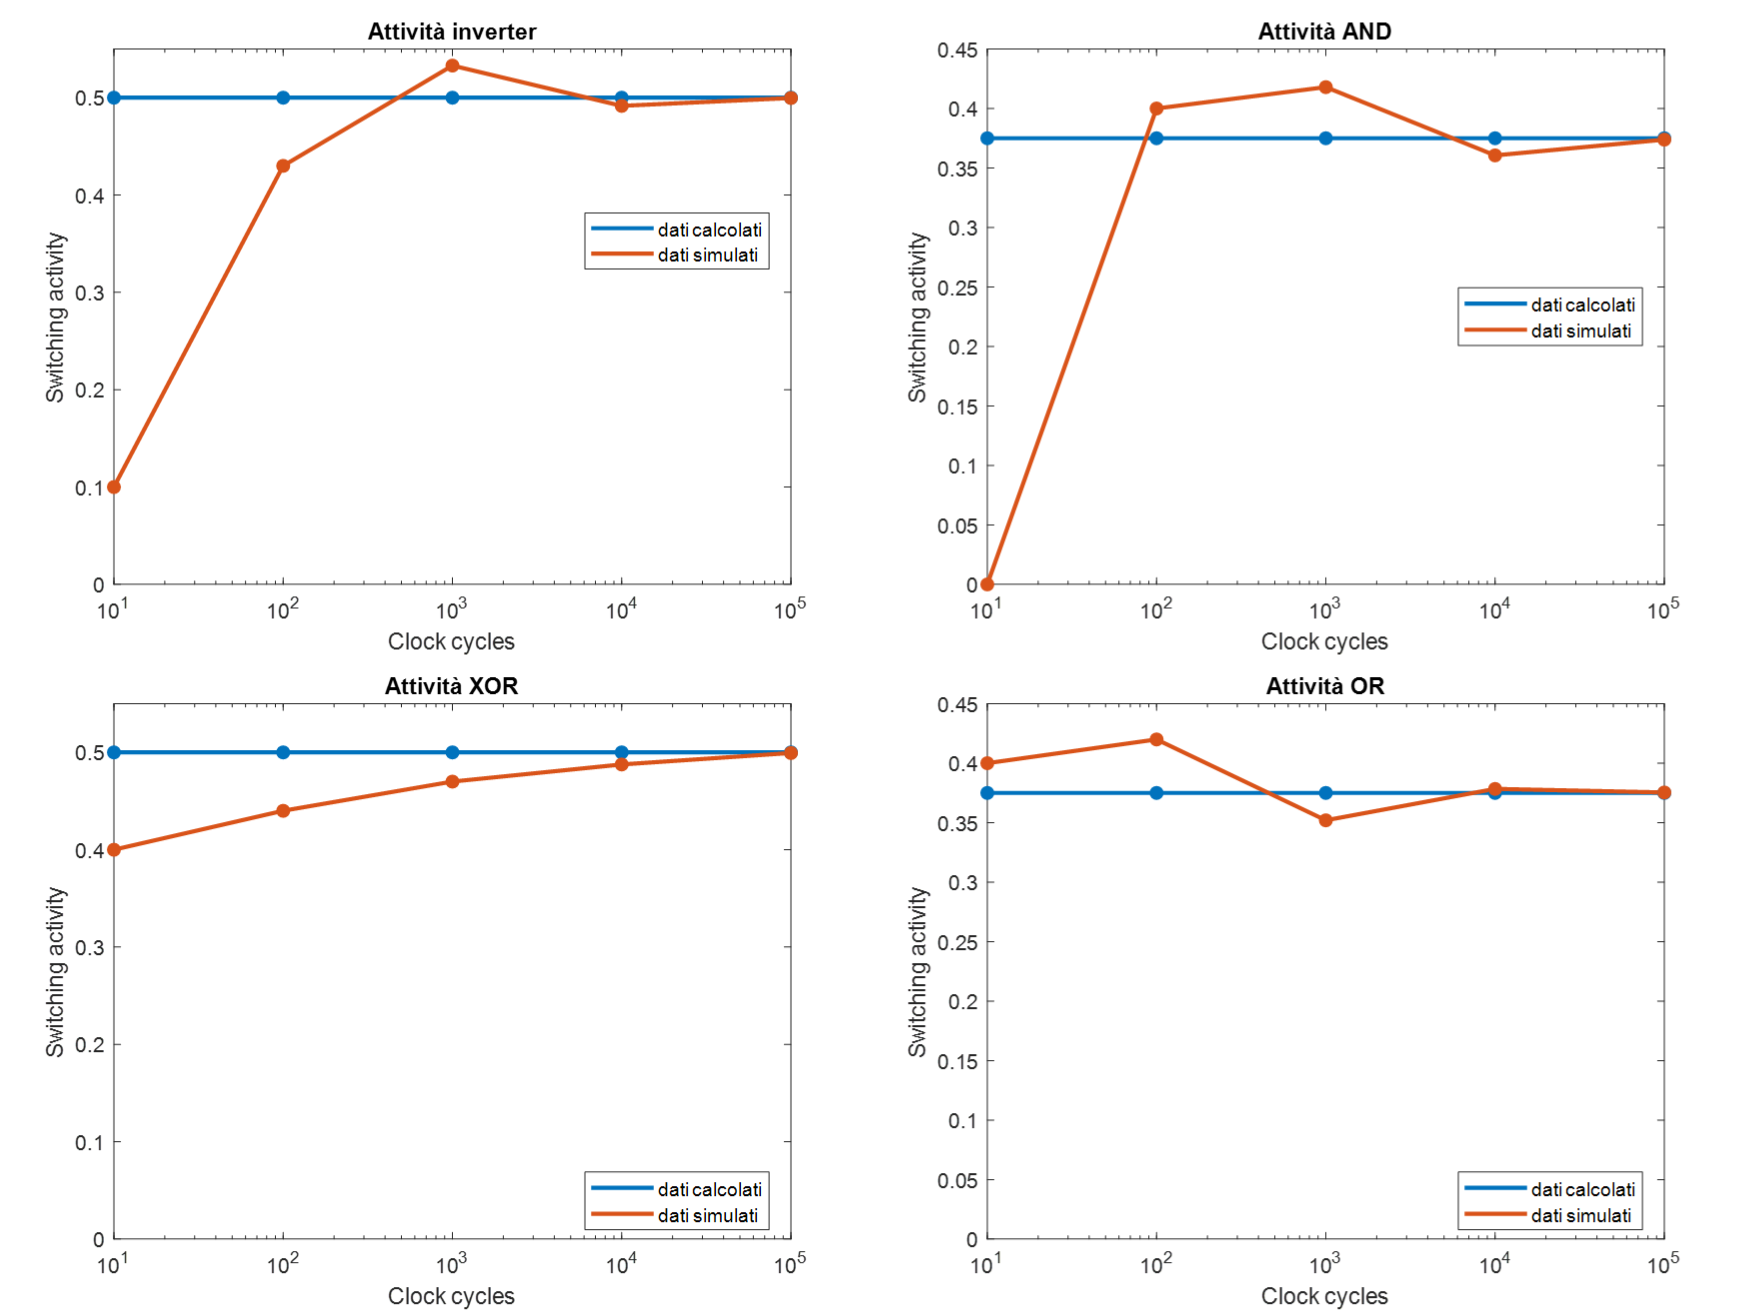
\includegraphics[width=15cm]{./img/Lab_1/Es_1/Grafici_Es_1.png}}
\\\\\\
Si osserva che all'aumentare del tempo di simulazione la stima 
dell'attività risulta a man mano più accurata. In particolare, 
nel caso analizzato, si osserva che per un numero di cicli di clock 
superiore a 10000, i dati sono confrontabili con quelli teorici.
\pagebreak

\section{Calcolo di probabilità e attività: half adder e full adder} % DA FINIRE
Dalle tavole di verità di Half Adder e Full Adder si ottengono le seguenti funzioni:
\\
\begin{itemize}
	\item \textbf{Half adder} \\
	S = A XOR B \\
	Cout = A AND B
	\item \textbf{Full adder} \\
	S = A XOR B XOR Cin \\
	Cout = A AND B AND Cin \\
\end{itemize}
Partendo dalle funzioni delle uscite è stato possibile ricavare le probabilità
associate alle uscite e le relative attività.
\\
\begin{itemize}
	\item \textbf{Half adder}\\\\
	$P(S=1) = P(A=1) \cdot ((1-P(B=1)) + P(B=1) \cdot (1-P(A=1))$ \\
	$P(Cout=1) = P(A=1) \cdot P(B=1)$ \\
	$A(S) = 2 \cdot P(S=1) \cdot (1-P(S=1))$ \\
	$A(Cout) = 2 \cdot P(Cout=1) \cdot (1-P(Cout=1))$ \\
	\item \textbf{Full adder} \\\\
	$P(S=1) = P(A=1) \cdot(1-P(B=1)) \cdot (1-P(Cin=1)) + \\ 
	          P(B=1) \cdot(1-P(A=1)) \cdot (1-P(Cin=1)) + \\
	          P(Cin=1) \cdot (1-P(A=1)) \cdot(1-P(B=1)) + \\
	          P(A=1) \cdot P(B=1) \cdot P(Cin=1)$	          
	$P(Cout=1) =$
	$A(S) =$
	$A(COut) =$
\end{itemize} 
\pagebreak

\section{MUX: generazione e propagazione di glitch}
L'obiettivo di questo esercizio è lo studio delle conseguenze 
introdotte dai ritardi delle porte, in particolare all'interno del
multiplexer nella seguente figura.
\\\\\
\centerline{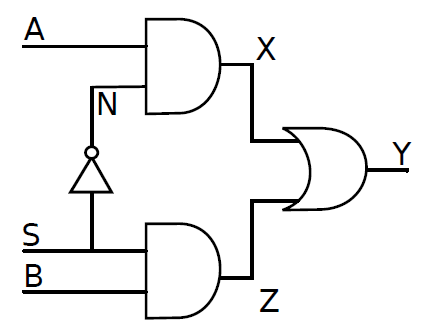
\includegraphics[width=5cm]{./img/Lab_1/Es_4/Mux.png}}
\\\\\
In questo caso particolare tutte le porte sono esenti da ritardi fatta
eccezione per l'inverter, caratterizzato da un ritardo di propagazione
di 0.1 ns.
\\
All'interno del file tb\textunderscore mux21\textunderscore
glitch.vhd è stato possibile identificare la combinazione 
dei segnali di ingresso con i quali il multiplexer è stato
testato.
\\\\
\begin{listato}
	\lstinputlisting{./code/Lab_1/Es_4/mux_input_delays.vhd}
\end{listato}
In particolare è possibile notare dal codice VHDL sopra riportato
che inizialmente gli ingressi assumono tutti un valore logico alto.
Dopo 1ns il segnale S commuta. L'uscita in un caso ideale non dovrebbe
presentare commutazioni.
\\
Si ipotizza che, a causa del ritardo di propagazione introdotto dall'
inverter, vi è un intervallo temporale in cui i nodi interni X e Z 
assumono entrambi un valore logico basso, portando quindi l'uscita a 0.
\\
Attraverso una simulazione ModelSim è stato possibile osservare
attraverso le waveforms il comportamento reale dei segnali. Il risultato
di tale simulazione è riportato nella seguente immagine.
\\\\
\centerline{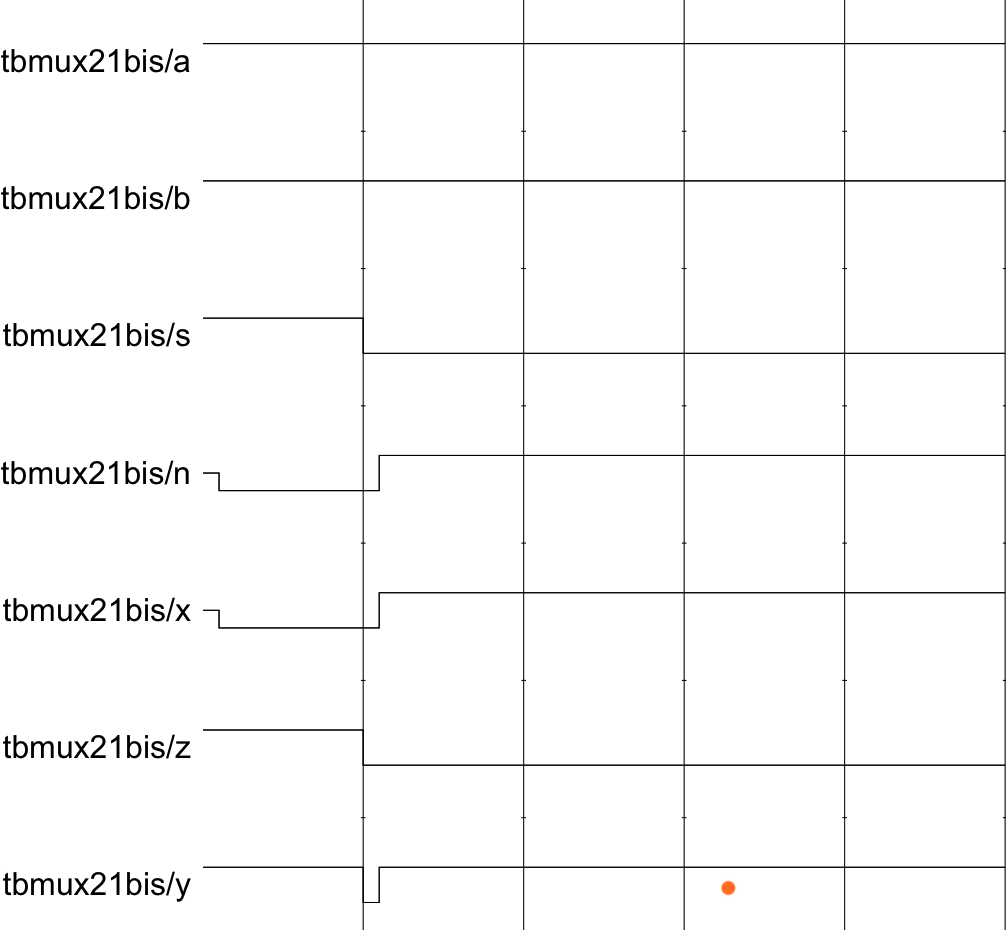
\includegraphics[width=10cm]{./img/Lab_1/Es_4/Glitch.png}}
\newpage
E' possibile visualizzare direttamente sulla waveform dell'uscita Y
il glitch causato dall'inverter. Tale comportamento è in linea con 
quanto atteso.
\\
Al fine di analizzare altre possibili combinazioni degli ingressi
che possano generare un glitch in uscita è stata realizzata una 
mappa di Karnaugh rappresentante la funzione logica del multiplexer.
\\\\\
MAPPA DI CARNO'
\\\\\
In particolare è possibile notare come, al fine di coprire la mappa
con il circuito in figura X, siano stati coperti i due implicanti
rappresentati sulla mappa stessa. In particolare il glitch analizzato
è dovuto ad una transizione degli ingressi che consegue in un passaggio
tra un implicante e l'altro. Tale problema potrebbe essere risolto
andando a coprire, in modo ridondante, con un terzo implicante per evitare
la transizione precedentemente trattata. 
\\
Tale ragionamento porta alla conclusione che l'unica combinazione in grado
di causare un glitch in uscita sia quella presa in analisi.
\\\\\
Essendo i glitch associati a commutazioni di nodi, questi portano un 
contributo aggiuntivo al consumo totale di potenza dinamica. In particolare
l'energia sprecata durante queste commutazioni spurie è la somma dei consumi
durante le due transizioni del segnale. Ciascuna delle due contribuisce alla
potenza secondo la seguente equazione:
\\\\
\centerline{$E = C \cdot V^{2}$}
\\\\
Dove C rappresenta la capacità di carico e V la tensione a cui viene caricata
tale capacità.
\\
Metà di tale contributo di energia è usata per caricare o scaricare la
capacità di carico associata all'uscita, mentre la restante parte viene
dissipata.
Di conseguenza il consumo di energia totale associato ad un glitch è 
dato da:
\\\\
\centerline{$E = 2 \cdot C \cdot V^{2}$}
\\\\

\section{Calcolo di probabilità e attività: contatore sincrono}
Nella prima parte di questo esercicio è stato analizzato il timing del blocco 
rappresentato nella figura seguente.
\\\\
\centerline{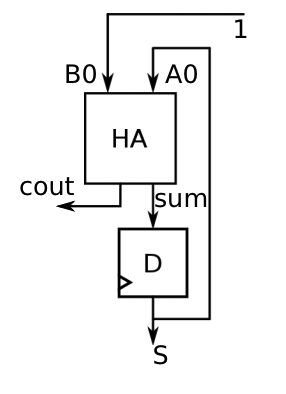
\includegraphics[width=3cm]{./img/Lab_1/Es_5/Sync_FA.png}}
\\\\
In particolare è stato possibile stabilire il suo comportamento atteso. 
Quando il segnale B0 è attivo alto, l'uscita S presenta una commutazione 
per ogni fronte sensibile del clock. Al contrario, quando B0 non è attivo, 
l'uscita non presenta alcuna commutazione.
\\
E' possibile utilizzare tali strutture per realizzare un contatore sincrono,
come mostrato in figura. In particolare i segnali di CEN e OVFL rappresentano
rispettivamente l'enable del contatore e il terminal count di questo.
\\\\
\centerline{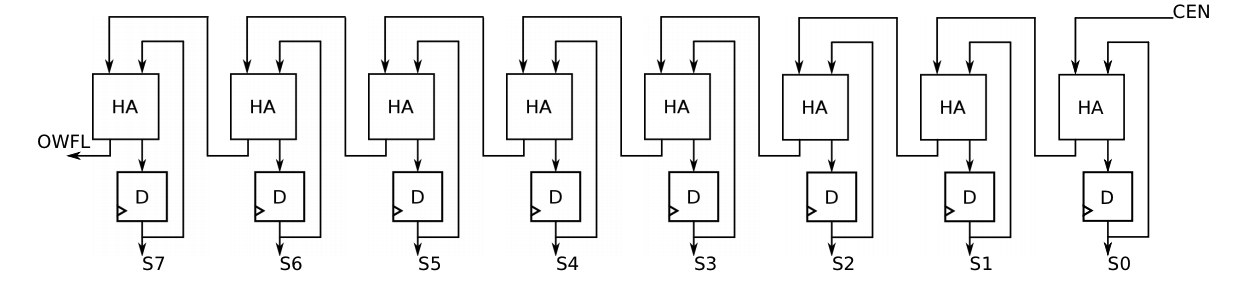
\includegraphics[width=20cm]{./img/Lab_1/Es_5/Counter.png}}
\\\\
Considerando infatti il comportamento delle uscite quando il segnale di 
enable è attivo si ottiene il seguente timing.
\\\\
TIMING CONTATORE FATTO DA NOI
\\\\
Dalle considerazioni fatte in precedenza è possibile stimare il numero
di commutazioni delle 8 uscite e del terminal count durante 
un intero ciclo di conta. Inoltre nella tabella seguente sono stati
aggiunti i dati ottenuti tramite simulazione attraverso ModelSim.
\\
\begin{center}
	\begin{tabular}{|c|c|c|}
	\hline
	Segnale & Transizioni stimate & Transizioni simulate \\ 
	\hline
	20 & 0.1 & 0 \\
	\hline
	200 & 0.43 & 0.40\\
	\hline
	2000 & 0.533 & 0.418\\
	\hline
	20000 & 0.4916 & 0.3606\\
	\hline
	200000 & 0.4997 & 0.3738 \\
	\hline
	200000 & 0.4997 & 0.3738 \\
	\hline
	200000 & 0.4997 & 0.3738 \\
	\hline
	200000 & 0.4997 & 0.3738 \\
	\hline
	200000 & 0.4997 & 0.3738 \\
	\hline
	200000 & 0.4997 & 0.3738 \\
	\hline
	\end{tabular}
\end{center}
\vspace{0.3cm}














\end{document}
